% This is samplepaper.tex, a sample chapter demonstrating the
% LLNCS macro package for Springer Computer Science proceedings;
% Version 2.20 of 2017/10/04
%
\documentclass[runningheads]{llncs}

\usepackage[T1]{fontenc}
\usepackage[utf8]{inputenc}
\usepackage{graphicx}
\usepackage{listings}
\usepackage{wrapfig}
\usepackage{hyperref}
\usepackage{stmaryrd}

\DeclareUnicodeCharacter{21D2}{$\Rightarrow$}
\DeclareUnicodeCharacter{2227}{$\wedge$}
\DeclareUnicodeCharacter{2260}{$\neq$}
\DeclareUnicodeCharacter{2265}{$\geq$}
\DeclareUnicodeCharacter{2264}{$\leq$}
\DeclareUnicodeCharacter{27F9}{$\Longrightarrow$}
\DeclareUnicodeCharacter{2987}{$\llparenthesis$}
\DeclareUnicodeCharacter{2988}{$\rrparenthesis$}

% redefined to give listings in tt font
\renewcommand{\lstinline}[1]{\texttt{#1}}

% Used for displaying a sample figure. If possible, figure files should
% be included in EPS format.
%
% If you use the hyperref package, please uncomment the following line
% to display URLs in blue roman font according to Springer's eBook style:
% \renewcommand\UrlFont{\color{blue}\rmfamily}

\begin{document}
%
\title{Marlowe: implementing and analysing financial contracts\thanks{Supported by IOHK.}}
%
%\titlerunning{Abbreviated paper title}
% If the paper title is too long for the running head, you can set
% an abbreviated paper title here
%
\author{
Pablo {Lamela Seijas}\inst{1} \and
Alexander Nemish\inst{1} \and
David Smith\inst{1} \and
Simon Thompson\inst{1,2}\orcidID{0000-0002-2350-301X}}
%
\authorrunning{P. Lamela Seijas, A. Nemish, et al.}

% First names are abbreviated in the running head.
% If there are more than two authors, 'et al.' is used.
%
\institute{IOHK, Hong Kong, \url{https://iohk.io} \\
\email{\{alexander.nemish, pablo.lamela, david.smith, simon.thompson\}@iohk.io} \and
School of Computing, University of Kent, UK\\
\email{s.j.thompson@kent.ac.uk}}
%
\maketitle              % typeset the header of the contribution
%



\begin{abstract}
The abstract should briefly summarize the contents of the paper in
150--250 words.

\keywords{First keyword \and Second keyword \and Another keyword.}
\end{abstract}
%
%
%


\section{Introduction}

Intro
\section{Marlowe overview SJT}

Introduce the main types and informal overview of execution. Contrast with Marlowe 1.3 (as in ISoLA paper). Embedding in Haskell? [All this stuff is in the tutorial already]

\section{Implementation of Marlowe on Cardano}

Marlowe is specified by an executable semantics written in Haskell, but to make it usable in practice to execute financial contracts, it needs to be implemented on a blockchain. In this section we explain how Marlowe is executed on the Cardano blockchain using an interpreter written in the Plutus programming language.

\subsection{Cardano and Plutus}

Cardano is a third-generation blockchain that solves the energy usage
issue by moving to an energy efficient \emph{Proof of Stake} protocol~\cite{Ouroboros-Genesis}.

Cardano aims to support smart contracs during its Shelley release in 2020.
Cardano smart contract platform is called \emph{Plutus}, and
it uses Haskell programming language to generate a form of $System F_{\omega}$,
called \emph{Plutus Core}, by extending GHC using its plugin
support~\cite[Section 13.3]{ghcusersguide}.

To implement Marlowe contracts we use the PlutusTx compiler,
which compiles Haskell code into serialized \emph{Plutus Core} code,
to create a Cardano \emph{validator script} that ensures the correct execution of the contract.
This form of implementation relies on the extensions to the UTxO model described in~\cite{PlutusPlatform}.


\subsection{Extended UTxO}

Cardano uses so called UTxO (unspent transaction outputs) model, similar to Bitcoin. LINK
It extends Bitcoin's model by allowing transaction outputs to hold a \emph{Data Script}.
As it sounds, it's just a serialized data intended to store a contract state.
This allows us to create complex multitransactional contracts.

In nutshell, it EUTxO models looks like this:

\begin{figure}[!h]
    \centering
    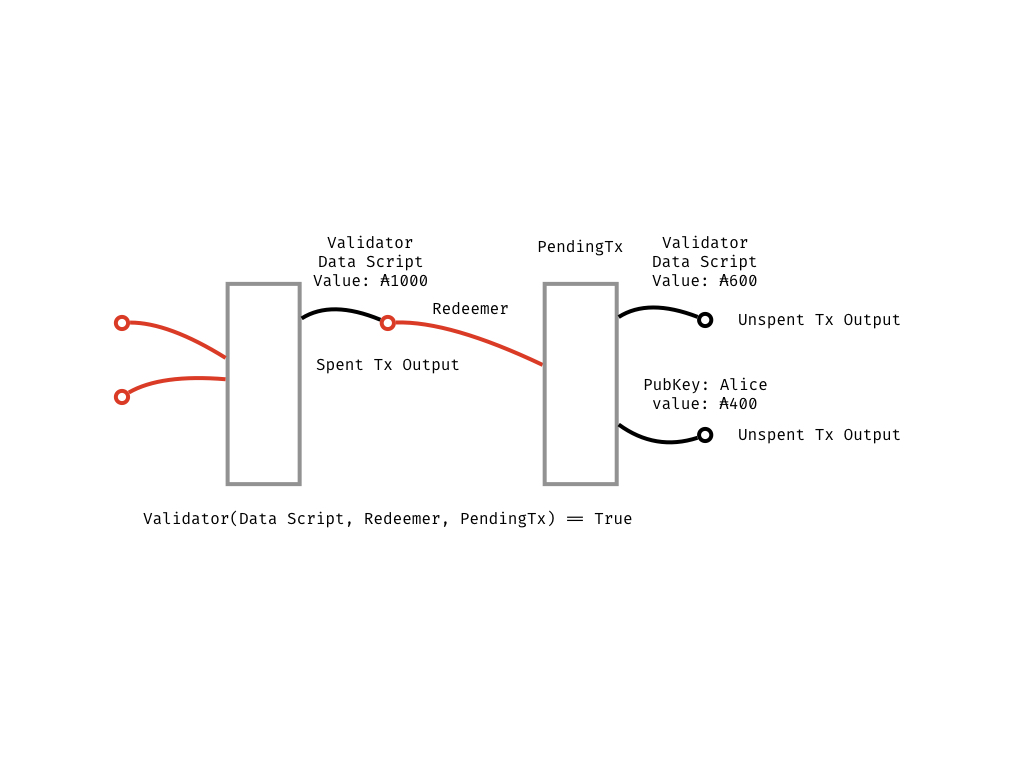
\includegraphics[width=4in]{figures/Marlowe3-Figures-003.jpeg}
    \caption{Cardano EUTx0 Model}
    \label{fig:eutxo}
\end{figure}

Black circles represent \emph{unspent transaction outputs}, and red lines show \emph{transaction inputs}
that reference existing \emph{transaction outputs}.
Each transaction output contains a \emph{Value} it holds, and is protected either by a \emph{public key},
or by a \emph{Validator}.

In order to spend an existing transaction output protected by a \emph{Validator},
one must create a transaction (\emph{PendingTx}) that has an \emph{input} that references the transaction output,
and contains such a \emph{Redeemer}, that

\begin{verbatim}
    Validator(Data Script, Redeemer, PendingTx)
\end{verbatim}
evaluates to $True$.

In order to spend a transaction output protected by a \emph{public key}, one must provide a valid signature
made with respective private key of the transaction public key.


\subsection{Design space}

There are several ways to implement Marlowe contracts on top of Plutus.
We could write a Marlowe to Plutus compiler that would convert
a particular Marlowe contract into a specific Plutus script.
Instead, we chose to implement an interpreter of Marlowe contracts.
This approach has a number of advantages:
\begin{itemize}
\item It is simple: we implement a single Plutus script that can be used for all Marlowe contracts,
thus making it easier to implement, review, and test what we have done.
\item It is close to the semantics of Marlowe, as sketched above and in more detail in~\cite{Marlowe:2018},
so making it easier to validate.
\item It means that the same implementation can be used for both on- and off-chain (wallet) execution of Marlowe code.
\item It allows client-side contract evaluation, where we reuse the same code
to do contract execution emulation (i.g. in IDE), and compile it to WASM/JavaScript on client side
(e.g.\ in Plutus Playground or Marlowe Playground).
\item Having a single interpreter for all (or a particular group of) Marlowe contracts allows
  to monitor the blockchain for these kinds of contract, if desired.
\item Finally, there is a potential to special-case this sort of script,
  and implement a specialized, highly effective interpreter in Cardano node itself.
\end{itemize}

Marlowe contract execution on the blockchain consists of a chain of transactions
where, at each stage, the remaining contract and its state are passed through the \emph{Data script},
and actions and inputs (i.e. \emph{choices} and \emph{money deposits}) are passed as
\emph{Redeemer}.
Each step in contract execution is a transaction that spends a Marlowe contract transaction output
by providing a valid input in $Redeemer$, and produces a transaction output
with a Marlowe contract as continuation (remaining contract).

We store a remaining contract in the \emph{Data script}, which makes it visible to everyone.
This simplifies contract reflection and retrospection.

\subsection{Contract lifecycle on extended UTxO model}

As we described above, the Marlowe interpreter is realised as a \emph{Validation script}.
We can divide the execution of a Marlowe Contract into two phases:
creation, and execution.

\paragraph{Creation}

Contract creation is realised as a transaction
with at least one script output,
with the particular Marlowe contract in the data script, and protected by the Marlowe validator script.
Note that we do not place any restriction on the transaction inputs, which could use any other transaction
outputs, including other scripts. This gives this model a great flexibility and composability.

\begin{verbatim}
data MarloweData = MarloweData {
    marloweState    :: State,
    marloweContract :: Contract
}
\end{verbatim}

Contract has a state

\begin{verbatim}
data State = State { accounts    :: Map AccountId Ada
                   , choices     :: Map ChoiceId ChosenNum
                   , boundValues :: Map ValueId Integer
                   , minSlot     :: Slot }
\end{verbatim}

where \emph{accounts} maps account ids to their balances, \emph{choices} stores user made choice values,
\emph{boundValues} stores evalutated \emph{Value}'s introduced by \emph{Let} expressions,
and \emph{minSlot} holds a minimal slot number a contract have seen (to avoid 'travels to the past')

It is possible to initialize a contract with a particular state, containing a number of deposits,
as shown in figure~\ref{fig:marlowe-init}.

\begin{figure}[!h]
\centering
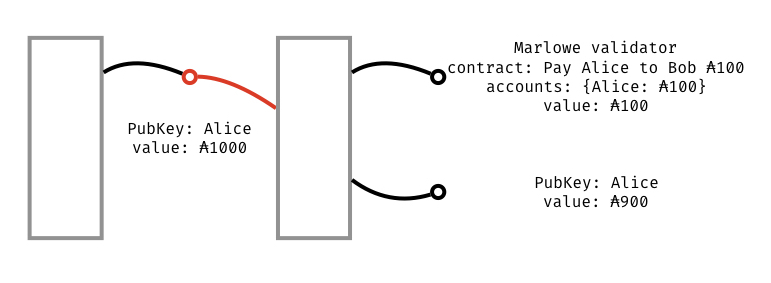
\includegraphics[width=1\textwidth]{figures/Marlowe3-Figures-002.jpeg}
\caption{Marlowe contract initialization}
\label{fig:marlowe-init}
\end{figure}

\paragraph{Execution}

Marlowe contract execution consists of a chain of transactions,
where the remaining contract and state are passed through the \emph{data script},
and input actions (i.e. \emph{choices}) are passed as \emph{redeemer scripts}.

Each execution step is a transaction that spends a Marlowe contract transaction output by providing
an expected input in a redeemer script,
and produces a transaction output with a Marlowe contract as continuation.

The Marlowe interpreter first validates the current contract state.
That is, we check that the contract locks at least what it should according
to contract balances (i.e. \emph{accounts} field in \emph{State}),
and all balances are strictly positive.

We have proven Isabelle proof assistant, that given a state with positive balances,
it's impossible to result in non-positive balances for all possible contracts and inputs.
LINK??

Then we compute expected transaction outcomes for given inputs, such as:
contract continuation, new state, and payments.

\begin{verbatim}
expectedTxOutputs = computeTransaction txInput marloweState marloweContract
\end{verbatim}

where

\begin{verbatim}
data TransactionInput = TransactionInput
    { txInterval :: SlotInterval
    , txInputs   :: [Input] }

data TransactionOutput =
    TransactionOutput
        { txOutWarnings :: [TransactionWarning]
        , txOutPayments :: [Payment]
        , txOutState    :: State
        , txOutContract :: Contract }
    | Error TransactionError

computeTransaction :: TransactionInput -> State -> Contract -> TransactionOutput
\end{verbatim}

Interpreter reduces a contract until it becomes quiescent, meaning it's either evaluates to \emph{Close},
or it expects a user input in \emph{When} construct.
This means that all \emph{Pay, If, Let, Close} constructs are evaluated immediately.

The function returns a new contract state, contract continuation, a list of warnings (such as partial payments),
and a list of expected payments (i.e. all evaluated \emph{Pay} constructs).

On-chain \emph{Validator} code cannot generate transaction outputs,
but can only validate whatever a user provides in a transaction.

Consider this simple zero coupon bond example.

\begin{verbatim}
When [ Case (Deposit aliceAccount alicePubKey (Constant 850_000_000))
    (Pay aliceAccount (Party bobPubKey) (Constant 850_000_000)
        (When
            [ Case
                (Deposit aliceAccount bobPubKey (Constant 1000_000_000))
                Close
            ] (Slot 200) Close
        ))] (Slot 100) Close
\end{verbatim}

Here we expect Alice to deposit 850 ada (850,000,000 lovelace) into her $aliceAccount$ before slot 100.
Otherwise, we \emph{Close} the contract.

If Alice deposits the money before slot 100, money immediately go to Bob,
by requiring a transaction output of 850 ada to Bob's public key address.
She must produce the following \emph{Redeemer} to satisfy Marlowe validator:

\begin{verbatim}
[IDeposit aliceAccount alicePubKey 850000000]
\end{verbatim}

Then Bob is expected to deposit 1000 ada into Alice's account before slot 200.
If he does, the contract is closed, and all remaining balances must be payed out
to their respective owners. In our case, 1000 ada must be payed to Alice.

\begin{figure}[!h]
    \centering
    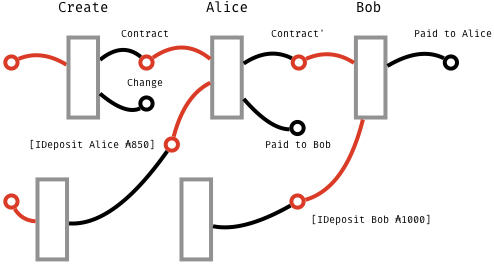
\includegraphics[width=1\textwidth]{figures/Marlowe3-Figures-004.jpeg}
    \caption{Zero Coupon Bond Contract}
    \label{fig:zero-coupon-bond}
\end{figure}

Note, that it's possible to provide multiple inputs at a time,
allowing to merge as many steps of a contract execution as necessary or possible.
This gives atomicity of some operations, and saves on transaction fees.

Sometimes it's necessary to just evaluate a contract in a given moment in time,
and not provide any inputs. Consider the following example:

\begin{verbatim}
If (SlotIntervalStart `ValueGT' 100)
    When [] (Slot 200)
        (Pay aliceAccount (Party bobPubKey) (Constant 1000))
    Close
\end{verbatim}

Let's say Alice has 1000 lovelace on her account, and Bob wants to receive the payment.
The payment could be obtained only after \emph{When} is timed out after slot 200.
Buy if we evaluate the contract after slot 200, \emph{If} reduces to \emph{Close}, and
Bob won't receive the payment. So he must evaluate the contract before slot 100 to
reduce \emph{If} to \emph{When}.
To do that he can spend the contract transaction output with empty list of inputs in \emph{redeemer}.
The he should do the same after slot 200 to receive the payment.


\paragraph{Ensuring execution validity}

Marlowe validator script checks that a transaction contains a valid continuation
output in case a contract is not closed, by checking output's validator hash, and state.

The continuation must have the same validator, hence the same hash of the validator script.
It should contain expected continuation contract and state, evaluated by \emph{computeTransaction}
function.

\paragraph{Closing a contract}

When a contract evaluates to \emph{Close}, and all remaining balances must payed out
to respective owners, removing the contract from the set of unspent transaction outputs.

\subsection{Further Work}

Cardano extends its ledger rules to support \emph{forging} of custom currencies and tokens,
effectively embedding support of Ethereum ERC-20 and ERC-721 contracts.
We are working on adding this \emph{multicurrency} support to Marlowe.

Simple token creation gives interesting possibilities of representing Marlowe contract parties with tokens.
Currently, parties are represented as public keys. We expect a valid signature for each input,
and do payments to respective addresses for party's public key.
In similar matter, we could check proofs of ownership of a particular token.

This allows us to tokenize contract participants, and abstract away concrete public key into contract \emph{roles}.
Thus, those roles could be traded independently of a contract.
Also, we can represent a role with multiple \emph{shares}, allowing automatic distribution of a payment
proportionally to a number of shares owned.

\section{Analysing Marlowe\label{sec:analysis}}

In this section, we give an overview of some of the work we have carried out with the aim of helping users be more confident that the Marlowe contracts they write do what they expect them to do.

We look at two complementary approaches: static analysis of concrete contracts (Section~\ref{subsec:static}) and formal verification of general properties about Marlowe (Section~\ref{subsec:verification}).

\subsection{Static analysis of contracts\label{subsec:static}}

For some properties, given a particular contract, a computer can decidably determine whether the contract satisfies the property and, in the cases when it does not, it can provide a counter-example.

For Turing-complete languages, this process is usually undecidable in the general case, and for Marlowe contracts it is often NP-complete in general. However, in practice, SMT (Satisfaction Modulo Theories) solvers are often able to solve moderately large instances of this problem reasonably efficiently.

Our implementation relies on the Haskell library SBV, which in turn relies on existing SMT solvers to check satisfiability of properties or finding counter-examples.

\subsubsection{SBV library}

SBV \cite{SBV} (SMT Base Verification) library provides a high-level API that allows developers to automatically prove properties about Haskell programs, among other functionalities.
The SBV library translates these properties to SMTLib queries, passes them to one or several SMT solvers, and translates the results back to the format in which the queries were written.

\paragraph{\texttt{SBV} monad.}

SBV provides a monad called \texttt{SBV} which encapsulates potentially unknown values to the program. A program that takes arguments wrapped with the \texttt{SBV} monad can be used with normal arguments and it can also be passed symbolic parameters when used as part of a property that is passed to the solver.
For example, the following function:

\begin{verbatim}
primeFactors :: SBV Integer -> SBV Integer -> SBV Bool
primeFactors x y = x .> 1 .&& y .> 1 .&& x * y .== 25723297
\end{verbatim}

\noindent
can be used both with normal integers and with symbolic parameters, that is, parameters whose concrete value is not specified and which the solver will try to replace with values that satisfy or falsify the property:

\begin{verbatim}
*Main> primeFactors 98 314
False
*Main> sat primeFactors
Satisfiable. Model:
    s0 = 6353 :: Integer
    s1 = 4049 :: Integer
*Main> primeFactors 6353 4049
True
\end{verbatim}

\paragraph{Limitations}

At the time of writing, there are some types of functions and data-types that SBV cannot translate to \texttt{SMTLib}. In particular, there are two that affected the way in which we use SBV with Marlowe and that prevent us from using the same version of the semantics for symbolic execution and normal execution.

Firstly, calls to recursive functions that are unbounded cannot be translated. As part of the process of converting functions to \texttt{SMTLib} terms, SBV unfolds them into a finite data-structure. For this reason, if the function is recursive and is not bounded by a non-symbolic value (a value that is known at the time of translation), the translation process will run out of memory.

Secondly, to the best our knowledge, SBV does not currently directly provide support for representing custom data types symbolically, except for zero-ary datatypes, i.e: enumerations.

In the following section, we explain how we worked around these limitations and give an overview of how we use SBV to avoid runtime problems with Marlowe contracts.

\subsubsection{Using SBV to analyse Marlowe Contracts}

Marlowe semantics are designed to use types to prevent many non-sensical contracts from being written. But there are potential problems which are harder to detect until runtime, for example, whether there will be enough money to issue all the payments declared in the contract. At this point it may already be too late to fix them, and particularly so in the case of blockchain. The Marlowe semantics represents these errors that can be found at runtime as \texttt{Warnings}.

The property that we have implemented using SBV library can be enunciated as: ``the given contract will not need to issue warnings at runtime no matter the inputs it receives''.

In order to achieve this, we implemented a symbolic version of the semantics that returns a list of the warnings produced by a trace (a list of transactions input to the contract):

\begin{verbatim}
warningsTraceWB :: Bounds -> SSlotNumber -> SList NTransaction
                -> Contract -> SList NTransactionWarning
\end{verbatim}

\noindent
where types that begin with \texttt{S}, like \texttt{SSlotNumber}, are abbreviations for the symbolic versions of types: in this case \texttt{SBV SlotNumber}.
The types that begin with \texttt{N} are \textit{nested} types, which we explain in the \textit{Custom datatypes} section below.

We can see that this version of the implementation takes two concrete parameters: \texttt{Bounds} (see \textit{Bounds for the state and the inputs} section below) and \texttt{Contract} (the contract we want to analyse); and two symbolic parameters: \texttt{SSlotNumber} (the initial slot number) and \texttt{SList NTransaction} (the input list of transactions); and it returns \texttt{SList NTransactionWarning} (a symbolic list of transaction warnings).

\paragraph{Custom datatypes}

As we mentioned before, SBV does not currently seem to support in general the use of custom datatypes. We do not need to represent the \texttt{Contract} type symbolically because we know its value at the time of analysis, but we still have a number of other types like \texttt{TransactionWarning} that are custom datatypes and we need to use.

Fortunately, SBV does support tuples and the \texttt{Either} type; combinations of those two give us essentially the same functionality as custom datatypes that are not recursive and have no type-parameters. We can represent all types that Marlowe requires as combinations of \texttt{Either} and tuples, with the exception of the \texttt{Contract} type, but we do not need a symbolic version of the \texttt{Contract} type.

\noindent
For example, the \texttt{TransactionResult} type:
\begin{verbatim}
data TransactionResult
 = TransactionProcessed [TransactionWarning]
                        [TransactionEffect]
                        State
 | TransactionError TransactionError
\end{verbatim}
\noindent
becomes the nested type synonym \texttt{NTransactionResult}:

\begin{verbatim}
type NTransactionResult =
  Either ([NTransactionWarning], [NTransactionEffect], NState)
         NTransactionError
\end{verbatim}

\noindent
Because working with nested types is much more error prone than working with the original data-types, we used Template Haskell \cite{sheard2002template} to implement functions that transform the custom datatypes into nested types and generate the appropriate conversion functions.

\paragraph{Returning non-symbolic \texttt{Contract} values}

In the non-symbolic semantics, each step typically takes a \texttt{Contract}, a \texttt{State}, and a set of \texttt{Input}s; and it returns an updated \texttt{State} and a remaining \texttt{Contract}.

This is a problem because values that rely on symbolic values have to be themselves symbolic. Moreover,  the resulting remaining \texttt{Contract} depends on the \texttt{Input}s and \texttt{State}, which are both symbolic.

We work around this problem by  modifying the signature of the function to receive a \textit{continuation function} instead, and instead of just returning a value, we return the result of applying the \textit{continuation function} to the result we were planning to return.

For example, the original type signature for the \texttt{apply} function was:

\begin{verbatim}
apply :: Environment -> State -> Input -> Contract -> ApplyResult
\end{verbatim}

\noindent
and the symbolic version of the \texttt{apply} function has the following signature:

\begin{verbatim}
apply :: SymVal a => Bounds
      -> SEnvironment -> SState -> SInput -> Contract
      -> (SApplyResult -> DetApplyResult -> SBV a) -> SBV a
\end{verbatim}

\noindent
where \texttt{DetApplyResult} contains the parts of \texttt{ApplyResult} that are not symbolic (like the \texttt{Contract}).

\paragraph{Bounds for the state and the inputs}

The recursion in the execution of the semantics is bounded by the \texttt{Contract}, and because the \texttt{Contract} is not a symbolic parameter, the translation will terminate.

However, in both the input and the \texttt{State} record there are several lists (representing finite maps) that are not explicitly bounded in the implementation. Some parts of the semantics are bounded by the length of these lists (or maps), such as the implementation of \texttt{Close} that refunds any remaining money in the contract accounts.
In order for the symbolic implementation to be finite, we need to find a bound for the length of these lists and maps.

With the current semantics of Marlowe, all the lists/maps in \texttt{State} and input can be bounded when looking at a particular contract. In particular, we can find out quite easily, by looking at the contract, how many parties there are, how many choice identifiers are used, how many accounts are used, and how many let binding identifiers are used.

It is less obvious that we can also set a bound for the input \texttt{Transaction} list as the maximum number of nested \texttt{When}s in the contract (for all the execution paths) plus one. We also provide a proof in Isabelle that shows that any longer list of transactions will result in an error (we discuss this in Section~\ref{subsubsec:bound_max_transaction_number}).

\subsection{Formal verification of semantics\label{subsec:verification}}

We can also use proof assistants to demonstrate that Marlowe semantics present certain desirable properties (like that money is preserved and returned to users by the end of the execution of any contract). In the same way, we can also use this technique to prove properties for particular contracts, or for particular contract snippets, templates, or classes of contracts.

Currently, we have translated the Haskell Marlowe semantics to Isabelle as closely as possible. The main differences between the Isabelle and the Haskell semantics are that:
\begin{itemize}
    \item The Isabelle semantics uses \emph{integers for identifiers} and the Haskell semantics uses strings. We do this because handling integers in Isabelle is easier and we only compare them for equality and order (their value is irrelevant).
    \item We use a \emph{custom implementation of maps and sets} that uses lists of tuples and lists of elements respectively. We do this because Isabelle already provides many theorems that are proven for lists, so it considerably facilitates the automation of certain proofs.
\end{itemize}

\subsubsection{Termination proof}

As part of the formalisation of the semantics, Isabelle proves termination automatically for most functions. The only function for which termination is not trivial is \texttt{reductionLoop}. The reason why Isabelle cannot infer termination for this function is that it repeatedly calls \texttt{reduceContractStep} until it returns \texttt{NotReduced}, so it requires proving that \texttt{reduceContractStep} will eventually do so.

The way we proved that this is the case was by establishing a measurment for the size of a pair of \texttt{Contract} and \texttt{State}. We defined such measurement as follows:

\begin{verbatim}
fun evalBound :: "State ⇒ Contract ⇒ nat" where
"evalBound sta cont = length (accounts sta) + 2 * (size cont)"
\end{verbatim}

\texttt{size} is a measurement already generated automatically by Isabelle for custom data types.

The reason why we need the number of accounts in the \texttt{State} for the measurement is that \texttt{reduceContractStep}, when called with the contract \texttt{Close}, will refund one of the accounts and the contract will remain as \texttt{Close}, so its \texttt{size} does not decrease.

And the reason why we multiply the size of the \texttt{Contract} by two is that the primitive \texttt{Deposit} may increase the number of accounts in the \texttt{State} by one, but it will also reduce the size of \texttt{Contract} by at least one. By multiplying the size of the \texttt{Contract} by two, the decrease in the \texttt{size} of the \texttt{Contract} compensates the increase in the \texttt{length} of the list of accounts and, thus, it ensures that the overall measurement \texttt{evalBound} will decrease even in that scenario.

\subsubsection{Valid state and positive account preservation}

Since we use lists of pairs of integers as maps in our \texttt{State}, there are some values that are allowed by the type definition of \texttt{State} still make no sense given what these lists represent:

\begin{enumerate}
    \item The lists of tuples are representing maps, so it does not make sense for two elements of the list to be tuples with the same first element (repeated keys).
    \item We want to minimise the number of ways in which a map can be represented as a list, so we require the tuples in the list to be sorted ascendingly by their first element. This allows us to use standard equality for comparing maps.
    \item We only expect accounts to store positive amounts money, so the second element of the tuples of the list of accounts must be a positive integer. Whenever an account becomes empty we just delete the account from the list.
\end{enumerate}

If a value of \texttt{State} satisfies the first two properties above we call it a \texttt{validState}. And we formalised the third property above as follows:

\begin{verbatim}
fun positiveMoneyInAccountOrNoAccount
             :: "AccountId ⇒ Token ⇒ Accounts ⇒ bool" where
"positiveMoneyInAccountOrNoAccount accId tok mlist =
    (case MList.lookup (accId, tok) mlist of
       None ⇒ True
     | Some x ⇒ x > 0)"
\end{verbatim}

For a state to have positive accounts, the above function must evaluate to \texttt{True} for any \texttt{AccountId} and \texttt{Token}.

We have proven that if all the three properties are true for a given input \texttt{State}, then the properties will also be true for the resulting output \texttt{State}, when processing any \texttt{Transaction} on any \texttt{Contract}.

\subsubsection{Quiescent result}

There is a class of combinations of \texttt{State} and \texttt{Contract} that will not evolve when passed to the semantics unless a matching \texttt{Input} is passed as well. We call these combinations of \texttt{Contract} and \texttt{State} \textit{quiescent}, and we define it as follows:

\begin{verbatim}
fun isQuiescent :: "Contract ⇒ State ⇒ bool" where
"isQuiescent Close state = (accounts state = [])" |
"isQuiescent (When _ _ _) _ = True" |
"isQuiescent _ _ = False"
\end{verbatim}

We have proven that, if an input \texttt{State} is valid and all accounts are positive, then the combination of \texttt{State} and \texttt{Contract} resulting from processing any transaction will always be quiescent.

\subsubsection{Money preservation and contract timeout}

One of the dangers of using smart-contracts is that a badly written one can potentially lock its funds forever. We want to avoid that feature in Marlowe altogether and, with that aim, we proved that Marlowe account system does not create or destroy any money. By the end of the contract, all the money paid to the contract must be distributed back, in some way, to a subset of the participants of the contract.

To ensure this is the case we proved two properties:

\paragraph{Money preservation}
Money is not created or destroyed by the semantics. We state this property as follows:

\begin{verbatim}
lemma computeTransaction_preserves_money :
"validAndPositive_state state
  ⟹ moneyInState state + moneyInInputs (inputs tra)
       = moneyInTransactionOutput state (inputs tra)
               (computeTransaction tra state contract)"
\end{verbatim}

The only consideration is that we only accept positive \texttt{Deposit}s, so we interpret money in \texttt{Deposit} inputs as the maximum of $0$ and the actual value specified in the \texttt{Deposit} input.

\paragraph{Timeout closes a contract}

For every Marlowe \texttt{Contract} there exists a slot number after which an empty transaction can be issued that will close the contract and refund all the money in its accounts.

A conservative upper bound for the expiration slot number can be calculated efficiently by using the function \texttt{maxTime} (or \texttt{maxTimeContract} in the Isabelle semantics).

We proved that this conservative upper bound works for every contract in a property stated as follows:

\begin{verbatim}
theorem timedOutTransaction_closes_contract :
"validAndPositive_state sta
 ⟹ iniSlot ≥ minSlot sta
 ⟹ iniSlot ≥ maxTimeContract cont
 ⟹ endSlot ≥ iniSlot
 ⟹ accounts sta ≠ []
 ⟹ isClosedAndEmpty
         (computeTransaction ⦇ interval = (iniSlot, endSlot)
                             , inputs = [] ⦈ sta cont)"
\end{verbatim}

\noindent

where \texttt{isClosedAndEmpty} is defined as follows:

\begin{verbatim}
fun isClosedAndEmpty :: "TransactionOutput ⇒ bool" where
"isClosedAndEmpty (TransactionOutput txOut) =
   (txOutContract txOut = Close
      ∧ accounts (txOutState txOut) = [])" |
"isClosedAndEmpty _ = False"
\end{verbatim}

Because the money is preserved and we know that there is an empty transaction that can be sent at any point after \texttt{maxTime} that will empty the accounts of the contract: we know that money will not be locked in the contract forever.

\subsubsection{Bound on the maximum number of transactions\label{subsubsec:bound_max_transaction_number}}

Another property of Marlowe is that any given finite \texttt{Contract} has an implicit finite bound on the maximum number of \texttt{Transaction}s that it accepts. This is a convenient property because:

\begin{itemize}
    \item It reduces the danger of Denegation of Service (DoS) attacks: because the number of valid inputs is limited, an attacker partcipant cannot arbitrarily block the contract by issuing an unbounded amount of useless \texttt{Transaction}s.
    \item It bounds the length of traces (the number of transactions) that symbolic execution (see Section~\ref{subsec:static}) needs to explore (more on this below).
\end{itemize}

We state the property as follows:

\begin{verbatim}
lemma playTrace_only_accepts_maxTransactionsInitialState :
"playTrace sl c l = TransactionOutput txOut
  ⟹ length l ≤ maxTransactionsInitialState c"
\end{verbatim}

\noindent
where \texttt{maxTransactionsInitialState} is essentially the maximum number of nested \texttt{When} in the contract plus one.

This property implies that any trace that is longer than this is guaranteed to produce at least one error. And because transactions that produce an error do not alter the state of the contract, such a list of transactions (trace) will be equivalent to a list of transactions that does not have the erroneous transaction.

In other words, for every list of \texttt{Transaction}s, there exists at least one list of \texttt{Transaction}s with length less or equal to \texttt{maxTransactionsInitialState} that has the same effect on the contracts.

Thus, we do not lose generality by only exploring traces with length of at most \texttt{maxTransactionsInitialState}, because any longer traces produce the same effect.

\section{The Marlowe Playground}

For Marlowe to be usable in practice, users need to be able to design and develop Marlowe contracts, and also to understand how contracts will behave once deployed to the blockchain, but without before actually deploying them.

The Marlowe Playground, a web-based tool that supports the interactive construction, revision, and simulation of smart contracts written in Marlowe, provides these facilities, as well as access to a static analysis of contracts (as described in the previous section), an online tutorial for Marlowe and a set of example contracts. The playground is available at \url{https://prod.meadow.marlowe.iohkdev.io/}.\footnote{Development of the playground is rapid, and the latest, unstable, version is also available at \url{https://alpha.marlowe.iohkdev.io/}.}

At the top level, the playground offers three panes: the main \emph{Simulation} pane, as well as panes for developing Marlowe contracts, embedded in \emph{Haskell} or using the \emph{Blockly} visual language.

\paragraph{Development}

On the simulation pane, ``pure'' Marlowe contacts can be developed: that is, contracts not embedded in a host language. The reason for doing this is two-fold:
\begin{itemize}
    \item There is a shallower learning curve for users who are new to Haskell or programming languages in general. The Marlowe constructs are quite simple, and there is no need, at least initially, to learn about Haskell syntax or even variables, functions etc.
    \item As we step through the execution of a contract in a simulation, the contract is reduced; it is very useful to be able to view, or even edit, the reduced contract during this execution.
\end{itemize}
As contracts become larger it makes sense to use another editor in the \emph{Haskell} pane. Here contracts can be written using facilities from \emph{Haskell} to abbreviate and make more readable the description of the contracts. These contracts can then be transferred as a pure Marlowe data structure into the simulation pane.

Contracts can also be written using Google's \emph{Blockly} visual programming language, as was earlier described in Meadow~\cite{isola-marlowe}. Blockly gives an easy way to introduce the concepts of Marlowe to users who have no programming knowledge, and in particular the editor gives users a set of options for each construct as the contract is built. Once a contract has been constructed in Blockly it is possible to transfer that contract to the simulation pane.%SJT Changed from "Marlowe editor".
It is also possible to transfer a Marlowe contract to Blockly for further editing.

\begin{wrapfigure}[9]{l}{0.25\textwidth}
    \vspace*{-0.3in}
    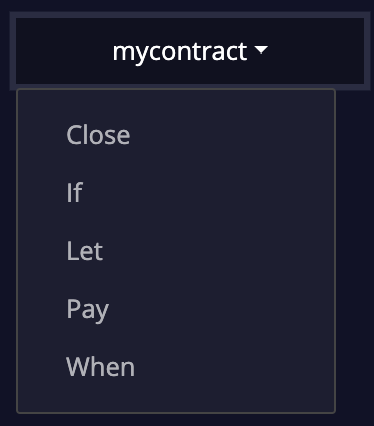
\includegraphics[width=0.25\textwidth]{hole_options.png}
\end{wrapfigure}

The Marlowe editor in the unstable version of the playground has an additional feature to aid writing contracts called holes. If we enter the contract \lstinline{?mycontract}
%SJT: enter it where?
we will be presented with a dropdown list of values that could be used.

In our case \lstinline{?mycontract} must be a \lstinline{Contract} of some sort, and so we are offered a choice of \lstinline{Contract} constructors from a dropdown list. If we choose \lstinline{Pay} then the Marlowe editor will automatically fill in a skeleton \lstinline{Pay} contract with new holes where we need to provide values.
\begin{verbatim}
    Pay ?accountId_1_1 ?payee_1_2 ?value_1_3 ?contract_1_4
\end{verbatim}
New options will be presented, one for each hole, and each will have a dropdown list of all the possible values.

\begin{wrapfigure}[6]{l}{0.25\textwidth}
    \vspace*{-0.3in}
    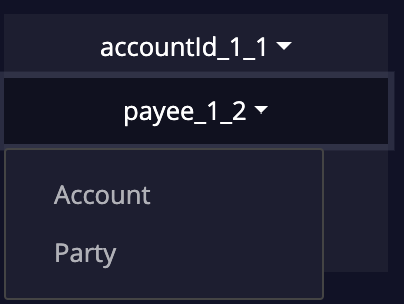
\includegraphics[scale=0.2]{hole_options_2.png}
\end{wrapfigure}
A complete contract can be written in this guided way with the user needing only to fill in strings and numbers by hand. This approach to writing holes in your code and ``asking'' the compiler what you could put in there is easy to implement in a DSL because there are very limited options, however is is also becoming popular with more complex languages such as Haskell and Idris.

Users can at any point save the current contract directly to a Github Gist, as well as being able to re-load contracts from Github Gists. There are also some demo contracts that can be loaded in their Haskell and Marlowe versions.

\paragraph{Simulation}

Contracts written in the Marlowe editor are parsed in real-time and if there are no errors (and no holes) then the contract is analysed to discover which actions a user could take to progress the contract. These actions are displayed in the ``Input Composer'' above the editor. Consider the following example contract:
\begin{verbatim}
    When [Case (Deposit (AccountId 0 "investor")
                        "guarantor"
                        (Constant 1000))
               Close]
         10
         Close
\end{verbatim}
In this case, the only action a user can take to progress the contract is to accept a deposit of 1000 ADA
%SJT: we need to sort out the Ada/Lovelance mismatch.
from the guarantor to the investor's account. Because of this, the playground can display this action in the input composer.

\begin{figure}[]
    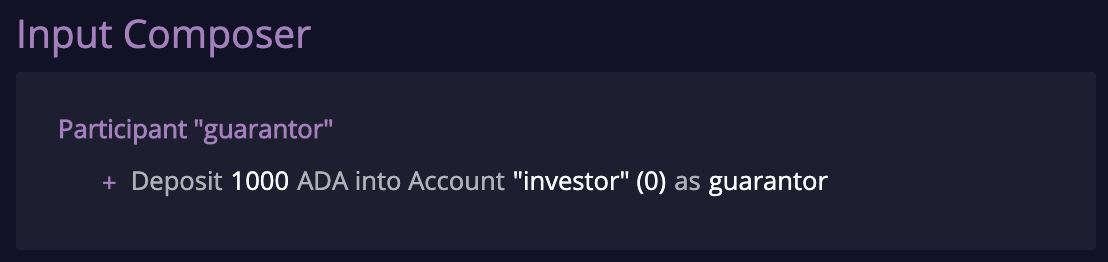
\includegraphics[width=1\textwidth]{input_composer.png}
\end{figure}

\noindent
The user can then choose to add this action to a transaction being prepared. Once the action is added other inputs become possible; these are displayed in the input composer, and again they can be added to the transaction being composed. In this way, multiple actions can be added to a transaction before it is applied.

\begin{figure}[]
    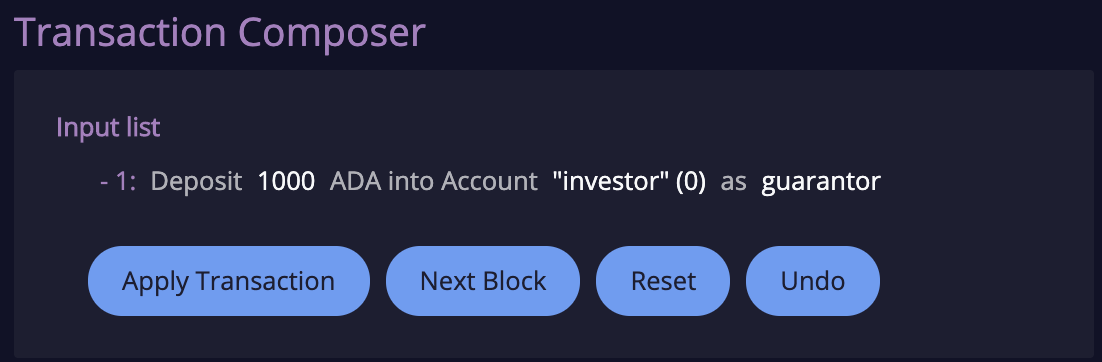
\includegraphics[width=0.8\textwidth]{tx_composer.png}
\end{figure}

\noindent
A user can then apply this transaction and in the example above this would result in the state pane showing a single payment and in addition the contract in the Marlowe editor will have been reduced to \lstinline{Close}.

At any point in the simulation the user can undo any steps made: in this particular case, they can undo the application of the transaction, and iteratively undo more steps. At any point they can also reset the contract to its initial state. This enables a user to apply transactions, see what the effect is, step back and apply a transaction with different actions and see how these differences affect the end result. They can also change the reduced contract to investigate variants of the original.

The final feature that we would like to present is the static analysis of contracts. As described in the previous section, it is possible to carry out a symbolic execution of a contract and then use a SMT solver to look for cases that could cause unwanted situations. The playground uses this to search for situations where contract execution would cause warnings. For example, suppose you write a contract that causes a payment of 450 Lovelace from Alice to Bob but the contract allows a situation where Alice has only deposited 350 Lovelace then the static analysis will find this and report it to the playground user.
\begin{figure}
    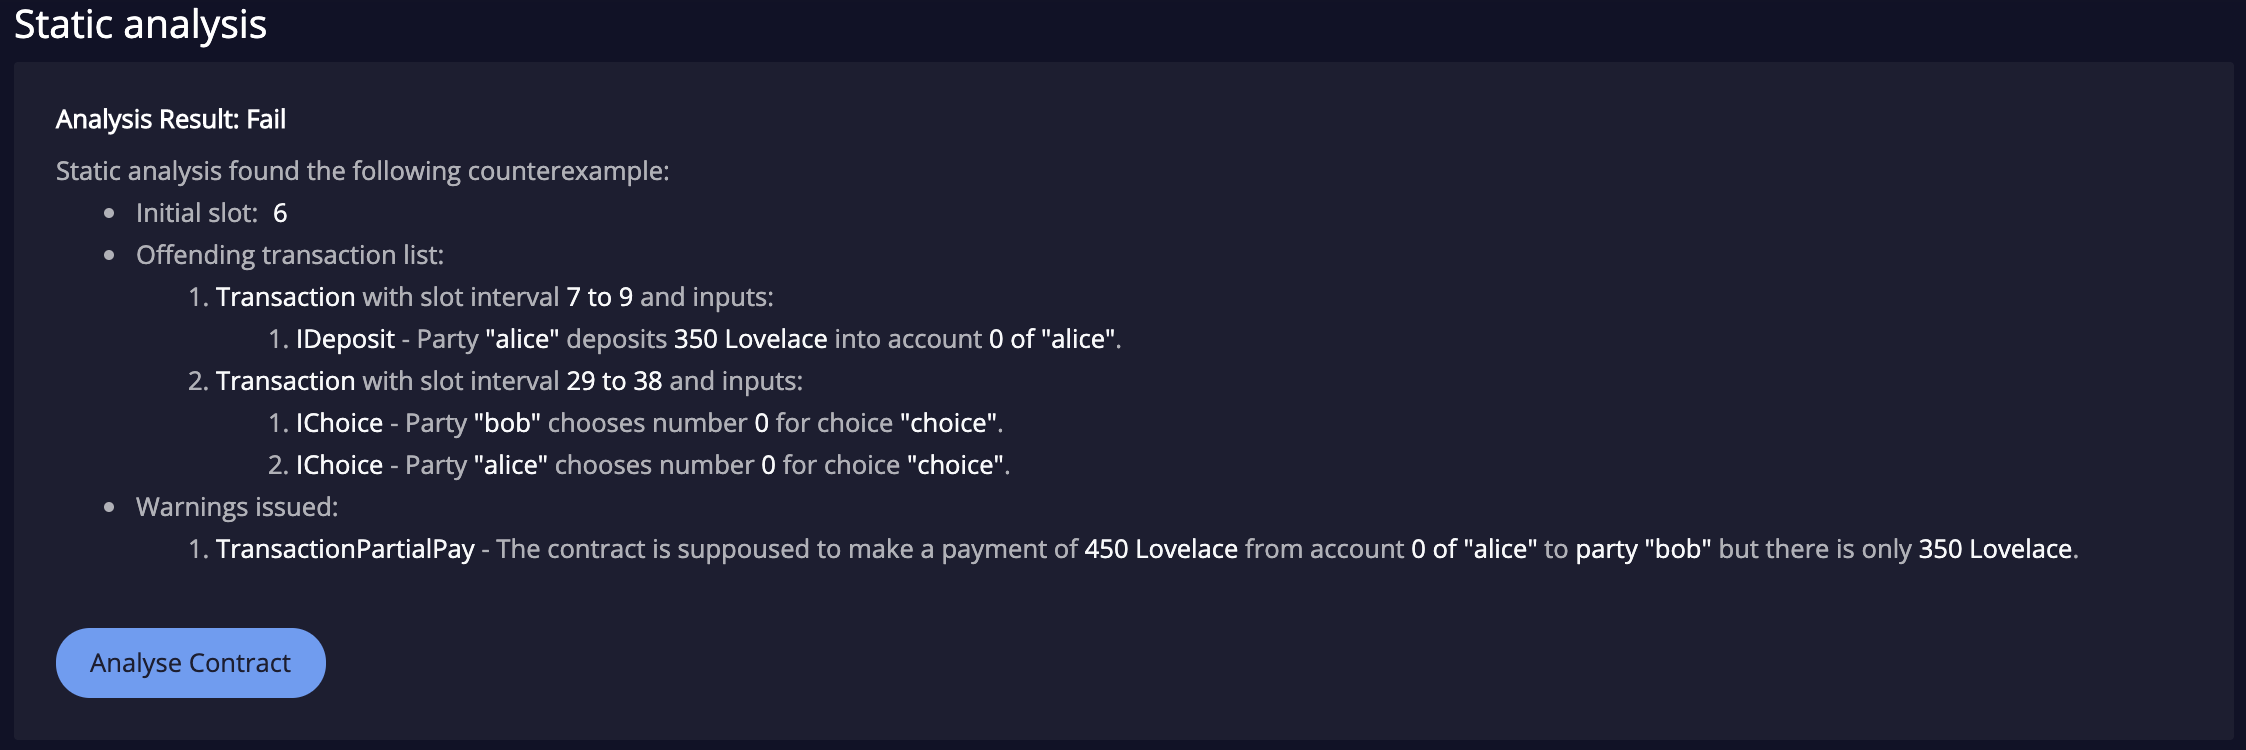
\includegraphics[width=1\textwidth]{static_analysis.png}
\end{figure}
\clearpage
\section{Related work}

Need to update from ISoLA paper \cite{isola-marlowe}.

\section{Future work and conclusions}

\section*{Left in for info \ldots}

\begin{figure}
% 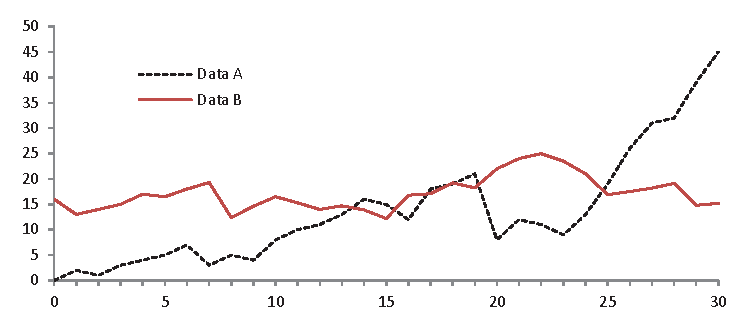
\includegraphics[width=\textwidth]{fig1.eps}
\caption{A figure caption is always placed below the illustration.
Please note that short captions are centered, while long ones are
justified by the macro package automatically.} \label{fig1}
\end{figure}


%
% ---- Bibliography ----
%
% BibTeX users should specify bibliography style 'splncs04'.
% References will then be sorted and formatted in the correct style.
%
\bibliographystyle{splncs04}
\bibliography{paper}
%
\end{document}
